\section{Recommendation Systems (25 points)}

\newcommand{\itt}[1]{\textnormal{item}_{#1}}
\newcommand{\user}[1]{\textnormal{user}_{#1}}
\newcommand{\cossim}{\operatorname{cos-sim}}
\newcommand{\argmin}{\operatornamewithlimits{argmin}}
\newcommand{\argmax}{\operatornamewithlimits{argmax}}

\textbf{Note}: Please use native Python (Spark not required) to solve this problem. If you run into memory error when doing large matrix operations, please make sure you are using 64-bit Python instead of 32-bit (which has a 4GB memory limit). 
\begin{center}
	{\footnotesize \ding{92} \hspace{1em} \ding{92} \hspace{1em} \ding{92}}
\end{center}


Consider a user-item bipartite graph where each edge in the graph between user $U$
to item $I$, indicates that user $U$ likes item $I$. We also represent the ratings
matrix for this set of users and items as $R$, where each row in $R$ corresponds to a user and each column corresponds to an item. If user $i$ likes
item $j$, then $R_{i,j}=1$, otherwise $R_{i,j}=0$. Also assume we have $m$ users
and $n$ items, so matrix $R$ is $m \times n$.

Let's define a matrix $P$, $m \times m$, as a diagonal matrix whose $i$-th diagonal
element is the degree of user node $i$, \emph{i.e.} the number of items that user $i$ likes. Similarly, a matrix $Q$, $n \times n$, is a diagonal matrix whose $i$-th
diagonal element is the degree of item node $i$ or the number of users that
liked item $i$. See figure below for an example.


\subquestion{(a) [4 points]} Define the non-normalized user similarity matrix $T = R*R^T$ (multiplication of $R$ and transposed $R$). Explain the meaning of $T_{ii}$ and $T_{ij}$ ($i \neq j$), in terms of bipartite graph structures (See Figure \ref{figpath}) (e.g. node degrees, path between nodes, etc.).

\begin{figure}[htbp]
\begin{center}
%\includegraphics[width=4.1in, height=4.1in]{useritem.eps}
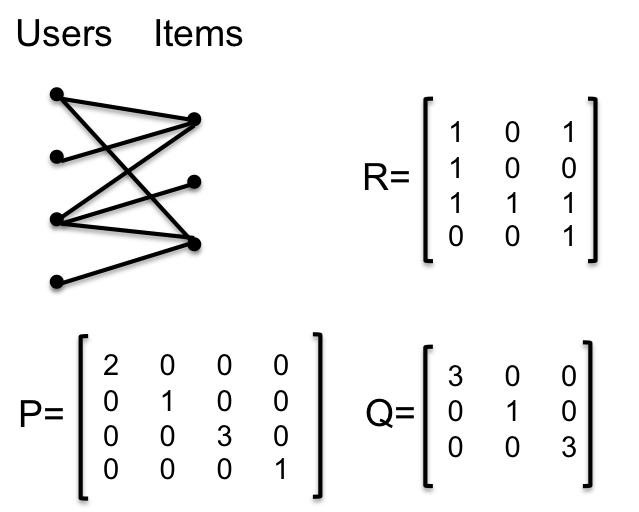
\includegraphics{user_item.png}
\caption{User-Item bipartite graph.}
\label{figpath}
\end{center}
\end{figure}

\vspace{0.4in}
\textbf{Cosine Similarity:} Recall that the cosine similarity of two vectors $u$
and $v$ is defined as:
\[ \textit{cos-sim(u,v)} = \frac {u \cdot v}{\|u\|\|v\|} \]

\subquestion{(b) [6 points]}

Let's define the \textit{item similarity matrix}, $S_{I}$, $n \times n$, such
that the element in row $i$ and column $j$ is the cosine similarity of \textit{item}
$i$ and \textit{item} $j$ which correspond to column $i$ and column $j$ of the matrix $R$. 
Show that $S_I = Q^{-1/2}R^TRQ^{-1/2}$, where $Q^{-1/2}$ is defined by $Q^{-1/2}_{rc} = 1/\sqrt{Q_{rc}}$ for all nonzero entries of the matrix, and $0$ at all other positions.

Repeat the same question for \textit{user similarity matrix}, $S_{U}$ where the
element in row $i$ and column $j$ is the cosine similarity of {\em user $i$} and
{\em user $j$}  which correspond to row $i$ and row $j$ of the matrix $R$. That is,
your expression for $S_U$ should also be in terms of some combination of $R$,
$P$, and $Q$. Your answer should be an operation on the matrices, in particular
you should not define each coefficient of $S_U$ individually.

Your answer should show how you derived the expressions.

\textit{(Note: To make the element-wise square root of a matrix, you may write it as matrix to the power of $\frac{1}{2}$.)}

\subquestion{(c) [5 points]}

The recommendation method using user-user collaborative filtering for user $u$, can be
described as follows: for all items $s$, compute $r_{u,s}=\Sigma_{x \in
\textit{users}}\cossim(x,u)*R_{xs}$ and recommend the $k$ items for which
$r_{u,s}$ is the largest.

Similarly, the recommendation method using item-item collaborative filtering for user $u$ can
be described as follows: for all items $s$, compute $r_{u,s}=\Sigma_{x \in
\textit{items}}R_{ux}*\cossim(x,s)$ and recommend the $k$ items for which $r_{u,s}$ is the largest.

Let's define the recommendation matrix, $\Gamma$, $m \times n$, such that
$\Gamma(i,j) = r_{i,j}$. Find $\Gamma$ for both item-item and user-user
collaborative filtering approaches, in terms of $R$, $P$ and $Q$. Your final answer should describe operations on matrix level, not specific terms of matrices. 

{\em Hint: For the item-item case, $\Gamma = RQ^{-1/2} R^TRQ^{-1/2}$.}

Your answer should show how you derived the expressions (even for the item-item case,
where we give you the final expression).

\subquestion{(d) [10 points]} In this question you will apply these methods to a real dataset. The data contains information about TV shows. More precisely, for 9985 users and 563 popular TV shows, we know if a given user watched a given show over a 3 month
period.

Use the dataset from \texttt{q4/data} within the bundle for this problem.

The folder contains:
\begin{itemize}
\item{\verb+user-shows.txt+} This is the ratings matrix $R$, where each row corresponds to a
user and each column corresponds to a TV show. $R_{ij} = 1$ if user $i$ watched the show
$j$ over a period of three months. The columns are separated by a space.
\item{\verb+shows.txt+} This is a file containing the titles of the TV shows, in the
same order as the columns of $R$.
\end{itemize}

We will compare the user-user and item-item collaborative filtering
recommendations for the 500\textsuperscript{th} user of the dataset. Let's call him Alex. (i.e. with Python's 0-based indexing, Alex=users[499].)

In order to do so, we have erased the first 100 entries of Alex's row in the
matrix, and replaced them by 0s. This means that we don't know which of the
first 100 shows Alex has watched. Based on Alex's behaviour on the other shows, we will give Alex recommendations on the first 100 shows. We will then see if our recommendations match what Alex had in fact watched.

\begin{itemize}
\item Compute the matrices $P$ and $Q$.
\item Using the formulas found in part (c), compute $\Gamma$ for the user-user
collaborative filtering. Let $S$ denote the set of the first 100 shows (the
first 100 columns of the matrix). From all the TV shows in $S$, which are the
five that have the highest similarity scores for Alex? In case of ties of similarity scores between two shows, choose the one with smaller index. Do not write the
index of the TV shows, write their names using the file \verb+shows.txt+.
\item Compute the matrix $\Gamma$ for the movie-movie collaborative filtering.
From all the TV shows in $S$, which are the five that have the highest similarity scores for
Alex? In case of ties between two shows, choose the one with smaller index.
Again, hand in the names of the shows and their similarity score.
\end{itemize}

For sanity check, your highest similarity score for user-user collaborative filtering should be above 900, and your highest similarity score for movie-movie filtering should be above 31. 

{\bf What to submit:} 
\begin{enumerate}[(i)]
\item Interpretation of $T_{ii}$ and $T_{ij}$ [4(a)]
\item Expression of $S_I$ and $S_U$ in terms of $R$, $P$ and $Q$ and accompanying explanation [4(b)]
\item Expression of $\Gamma$ in terms of $R$, $P$ and $Q$ and accompanying explanation [4(c)]
\item The answer to this question should include the followings: [4(d)]
\begin{itemize}
\item The \textbf{names} of five TV shows that have the highest similarity scores for Alex for the user-user collaborative filtering (no need to report the similarity scores)
\item The \textbf{names} of five TV shows that have the highest similarity scores for Alex for the item-item collaborative filtering (no need to report the similarity scores)
\item Upload the source code via Gradescope
\end{itemize}
\end{enumerate}